\hypertarget{PB3D_8f90}{}\section{/opt/\+P\+B3\+D/\+P\+B3D.f90 Program Rerefence}
\label{PB3D_8f90}\index{/opt/\+P\+B3\+D/\+P\+B3\+D@{/opt/\+P\+B3\+D/\+P\+B3\+D}}



Peeling Ballooning in 3D. 

\begin{DoxyAuthor}{Author}
Toon Weyens, Contact\+: \href{mailto:weyenst@gmail.com}{\tt weyenst@gmail.\+com} 
\end{DoxyAuthor}
\begin{DoxyVersion}{Version}
2.\+33 
\end{DoxyVersion}
\begin{DoxyDate}{Date}
2012-\/2018 
\end{DoxyDate}
\begin{DoxyCopyright}{Copyright}
G\+NU General Public License. 
\end{DoxyCopyright}
\begin{DoxySeeAlso}{See also}
References\+: \cite{weyens2014theory} \cite{Weyens2017PB3D} 
\end{DoxySeeAlso}


Definition at line 27 of file P\+B3\+D.

Here is the call graph for this function\+:\nopagebreak
\begin{figure}[H]
\begin{center}
\leavevmode
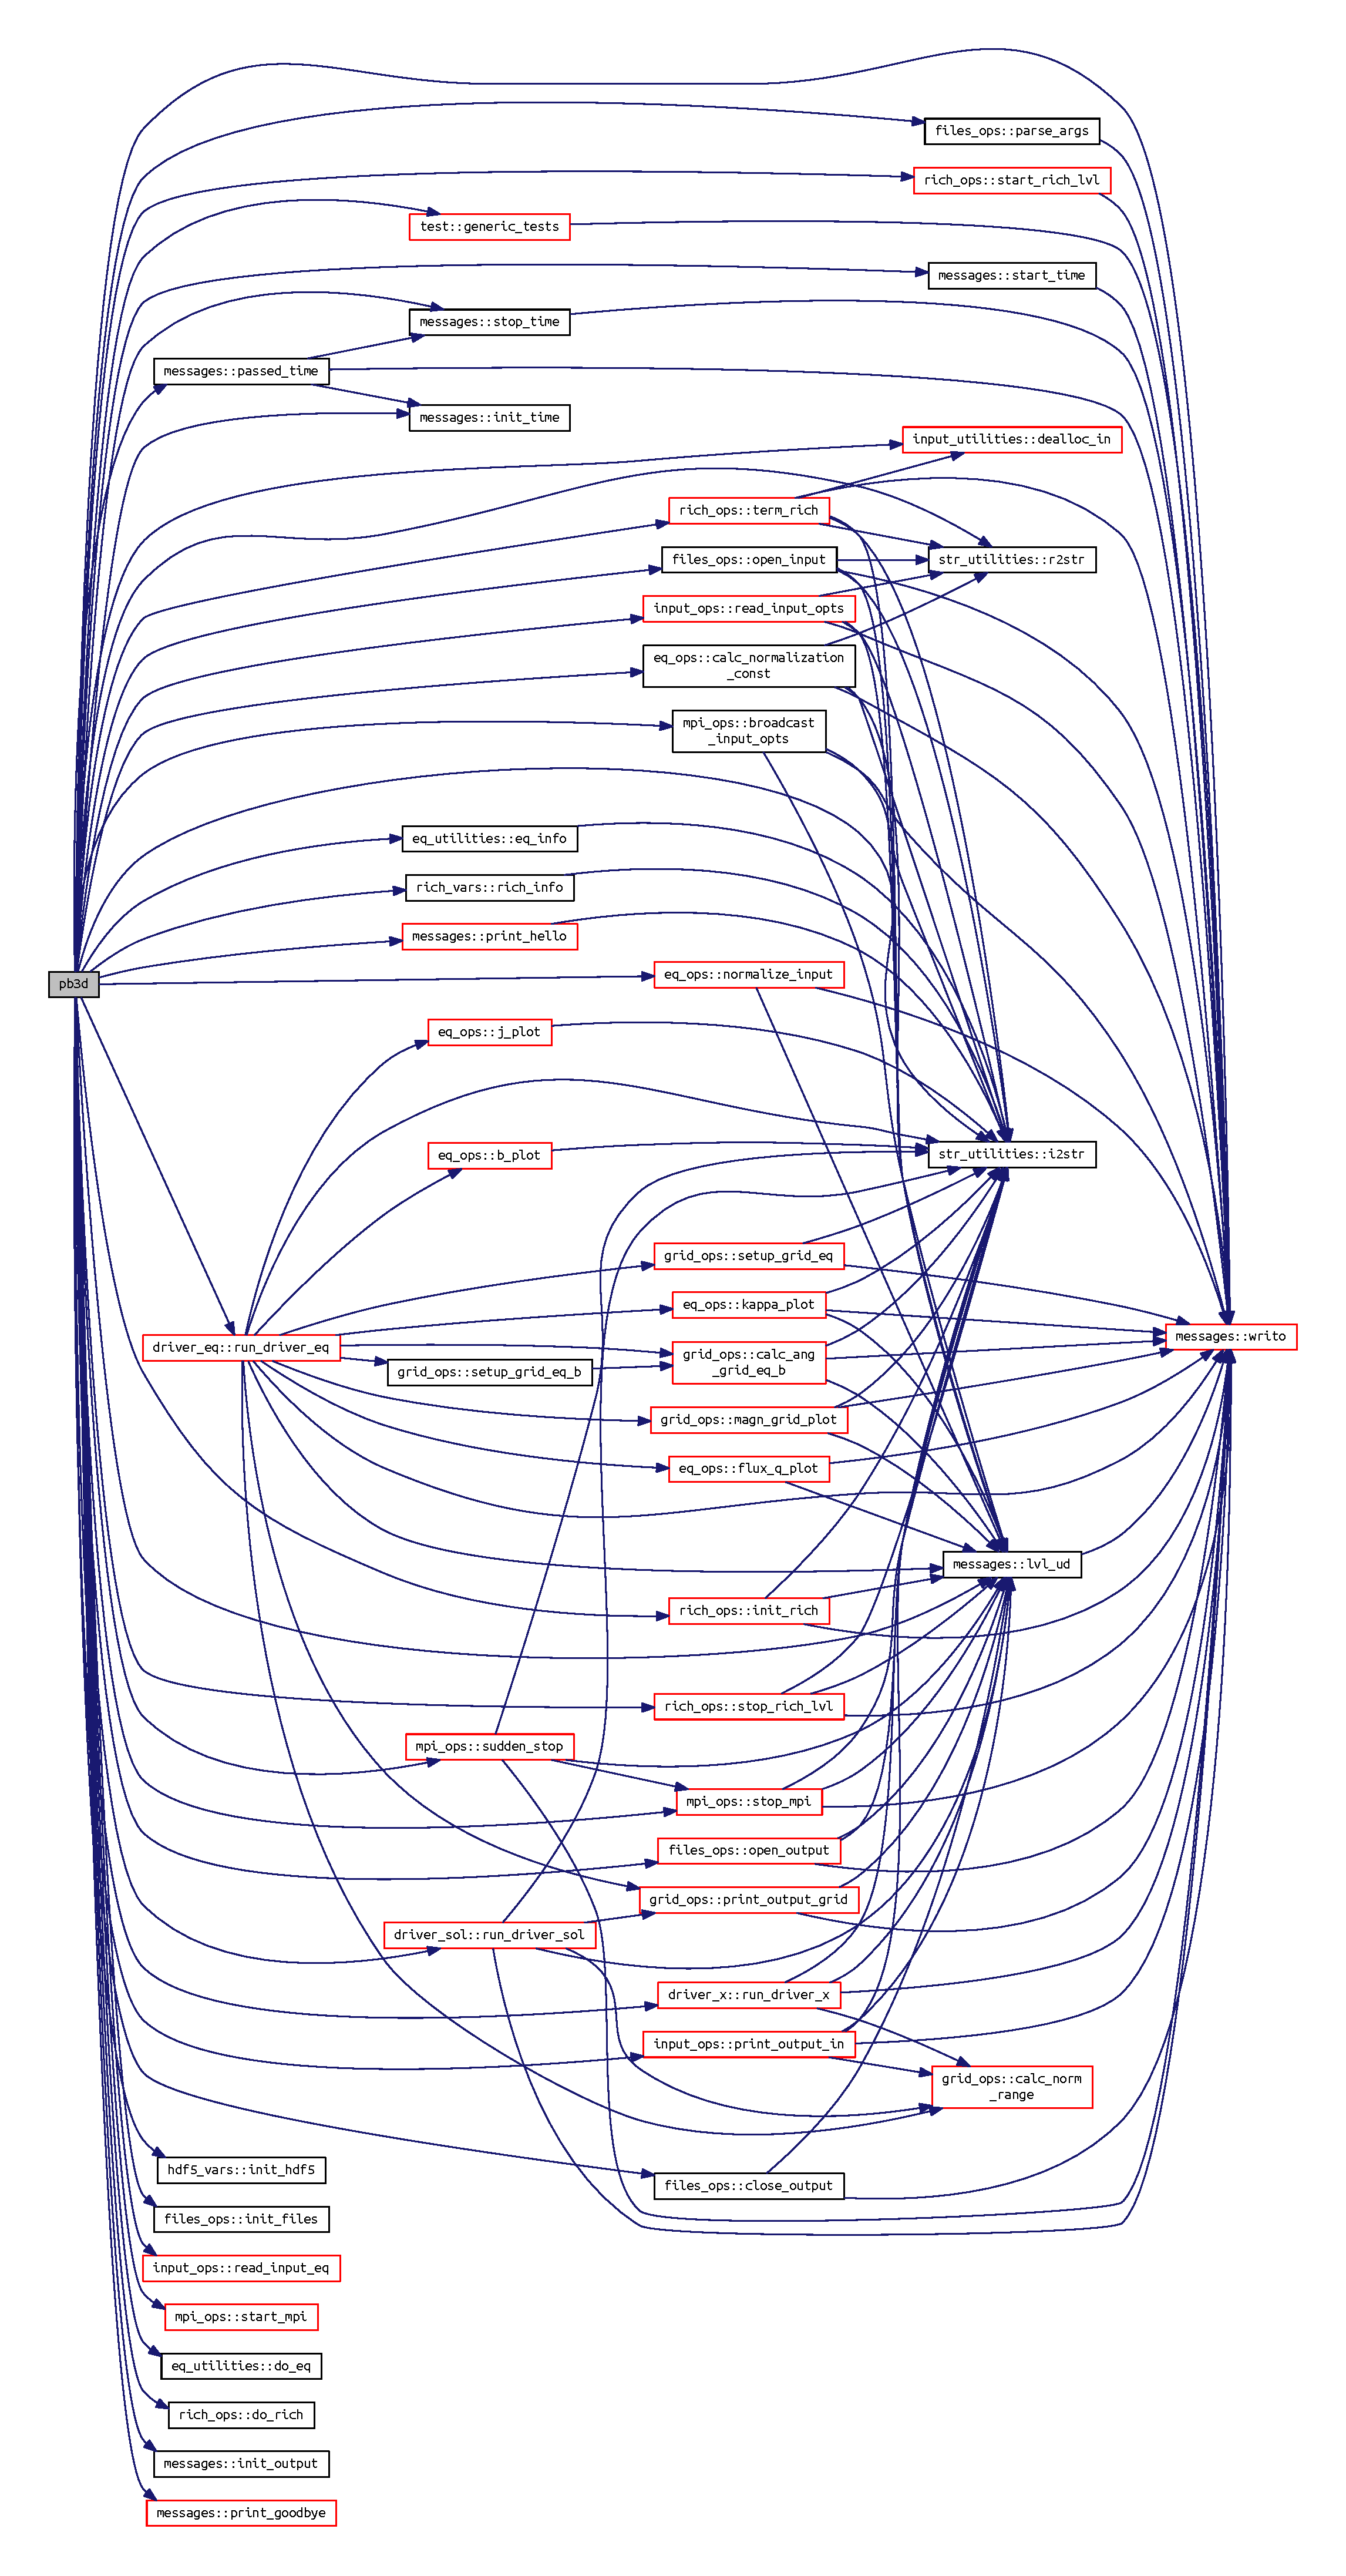
\includegraphics[height=550pt]{PB3D_8f90_afaee01f014ab3398eecac996b2795fd2_cgraph}
\end{center}
\end{figure}
